\section{Numerical experiments}\label{sec:numerics}

In this section we numerically verify the properties of the
constructed scheme $TM^{n-2}R$, where $M$ is an SSPRK($s,q,p$) and
$R$ and $T$ are its associated SSP starting and stopping schemes from
Section~\ref{subsec:starting_finishing}.
Specifically, we use a convergence study to show that the procedure
attains order $q$.  We also demonstrate on Burgers' equation that the
SSP coefficient accurately measures the maximal stepsize for which the
methods are strong stability preserving.

For simplicity we denote the multi-method $TM^{n-2}R$ procedure as the
\emph{ESSPRK-scheme}.

\subsection{Convergence study}\label{subsec:convergence}
We consider the nonlinear ODE
\begin{equation}\label{eq:conv_eq}
    u'(t) = -\frac{3}{2}u^{2}(t), \quad t \in [0,1], \quad \text{with } u(0) = 10,
\end{equation}
and exact solution $u(t) = 10/(15t + 1)$.
We solve the initial value problem \eqref{eq:conv_eq}
using an ESSPRK-scheme where $M$ is an 
ESSPRK($s,q,p$) method for $q = 3, 4$ and $p = 2$.
%The stages of the permutation methods were kept as low as possible, thus 
%we use two stages for a third-effective order method $M$ and four stages for 
%a fourth-effective order method. 
The solution is computed for using $N = 50 \cdot 2^{k}$ time steps for
$k = 0, 1, 2, \dots, 6$.
% and 
%hence the time-step used is $\Dt = \tfrac{1}{N} = \tfrac{2^{(1-k)}}{100}$ 
%for each computation. 
The error at $t=1$ between the exact solution and the approximation with respect 
to time-step is shown in Figure~\ref{fig:conv_study} on a logarithmic scale.
The convergence study was performed for various number of stages $s$ and the results 
show that the ESSPRK-scheme attains an order of accuracy equal to the effective order of 
method $M$.
It is important in doing this sort of convergence study that the
effective order can only be obtained after the finishing method is
applied.
Intermediate steps will typically only be order $p$ accurate (the classical
order of the main method).
Finally, we note that for a fixed time-step increasing the number of stages
generally decreases the error constant.

\begin{figure}
	\centering
     \subfloat[SSPRK($s,3,2$)]{\label{fig:conv_study_a}
     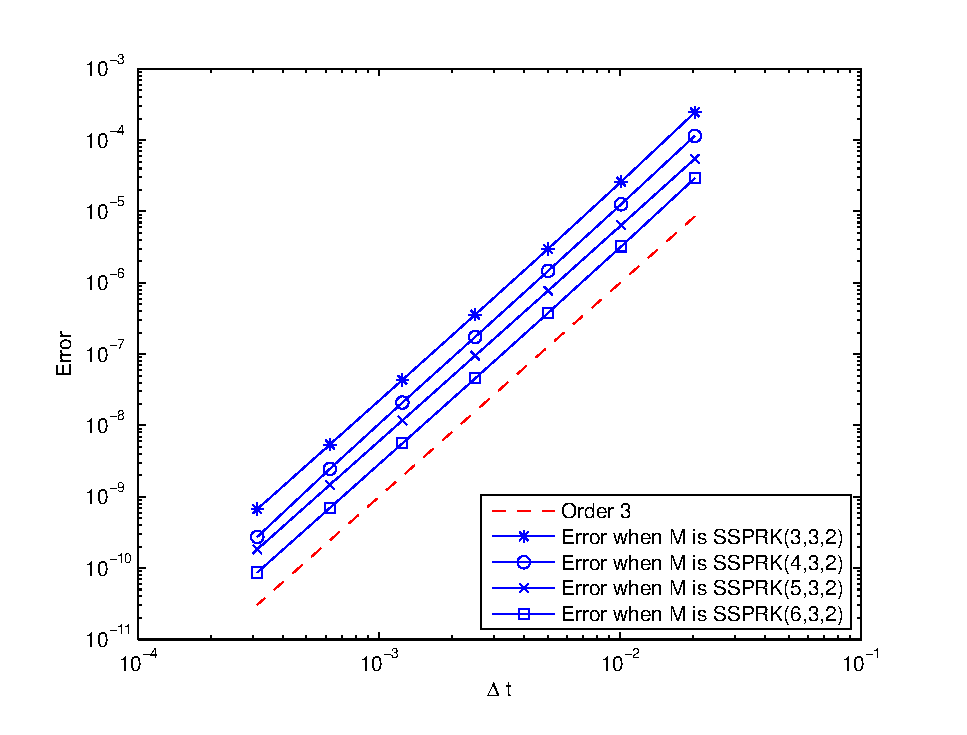
\includegraphics[width=0.5\textwidth]{Pictures/convergence_3rd_ord}}
     \subfloat[SSPRK($s,4,2$)]{\label{fig:conv_study_b}
    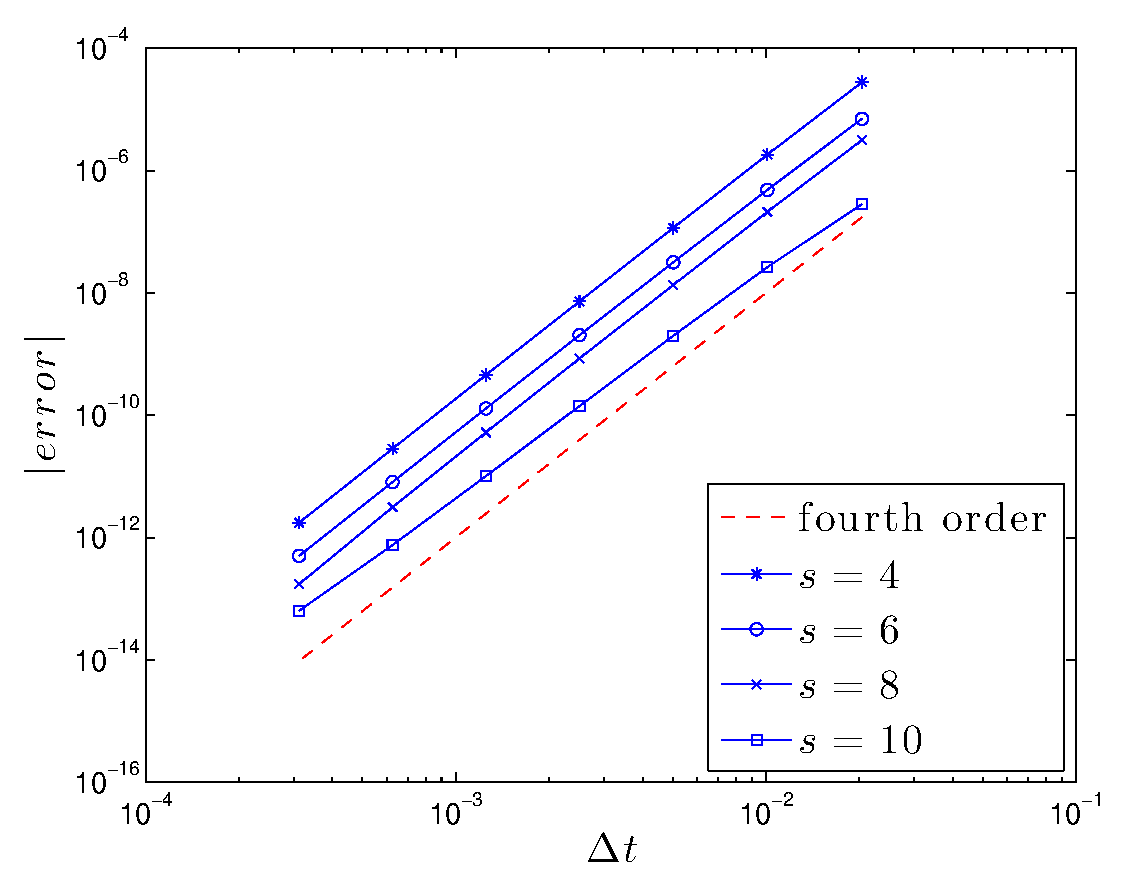
\includegraphics[width=0.5\textwidth]{Pictures/convergence_4th_ord}}
    \caption{Convergence of $TM^{n-2}R$ Runge-Kutta scheme when (a) $M$ 
    is an SSPRK($s,3,2$) method and (b) $ M $ is an SSPRK($s,4,2$) method.}
    \label{fig:conv_study}
\end{figure}


\subsection{Burgers' equation}\label{subsubsec:burgers}

The inviscid Burgers' equation consists of the hyperbolic conservation law
\begin{equation}\label{eq:HCL}
    U_{t} + f(U)_{x} = 0,
\end{equation}
when the flux function $f(U) = \frac{1}{2}U^{2}$. 
We consider initial data
%\begin{equation}\label{eq:burgers_IC}
    $U(0,x)  = \frac{1}{2} - \frac{1}{4}\sin{\pi x}$,
%\end{equation}
on a periodic domain $x \in [0,2)$.
The solution advances to the right where it eventually exhibits a shock. 
We perform a semi-discetisation of $f(U)_{x}$ using an upwind approximation 
\textbf{[Cite sth, Laney or LeVeque's red book?]}
\yianniscomment{This appears in this reference. I don't think LeVeque } that gives
\begin{equation}\label{eq:burgers_flux}
    f(U)_{x} \approx \frac{1}{\Dt}\bigl(f(U_{i}) - f(U_{i-1})\bigr).
\end{equation}
\colintodo{so much wrong with this sentence!}
\yiannistodo{I see your point. I wanted to refer to the full scheme (FE + TVD spatial discr.) which is SSP}
\sout{
The above time discretisation is SSP when coupled with Forward Euler method
}
The spatial discretization is total-variation-diminishing (TVD) when
coupled with Forward Euler method under time restriction
$\Dt \leq {\Dt}_{\text{FE}} = (1 / \|U(0,x)\|_{\infty}) \Delta x$
\textbf{[Cite]}.
The SSP theory predicts that using a time-discretization with a SSP
coefficient $\sspcoef$, the solution will be TVD for $\Dt \leq
\sspcoef {\Dt}_{\text{FE}}$.


\begin{figure}[t!]
    \centering
    \subfloat[$\sigma = 6.0$]{\label{fig:burgers_cont_a}
      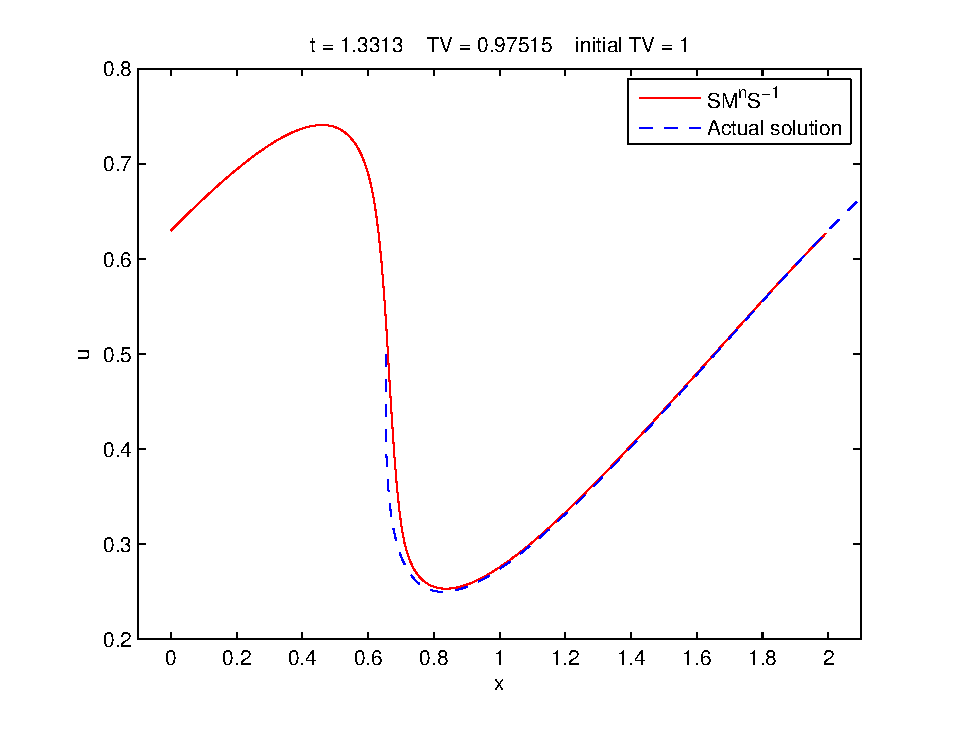
\includegraphics[width=0.5\textwidth]{Pictures/burgers_cont_tvd}}
    \subfloat[$\sigma = 6.68$]{\label{fig:burgers_cont_b}
      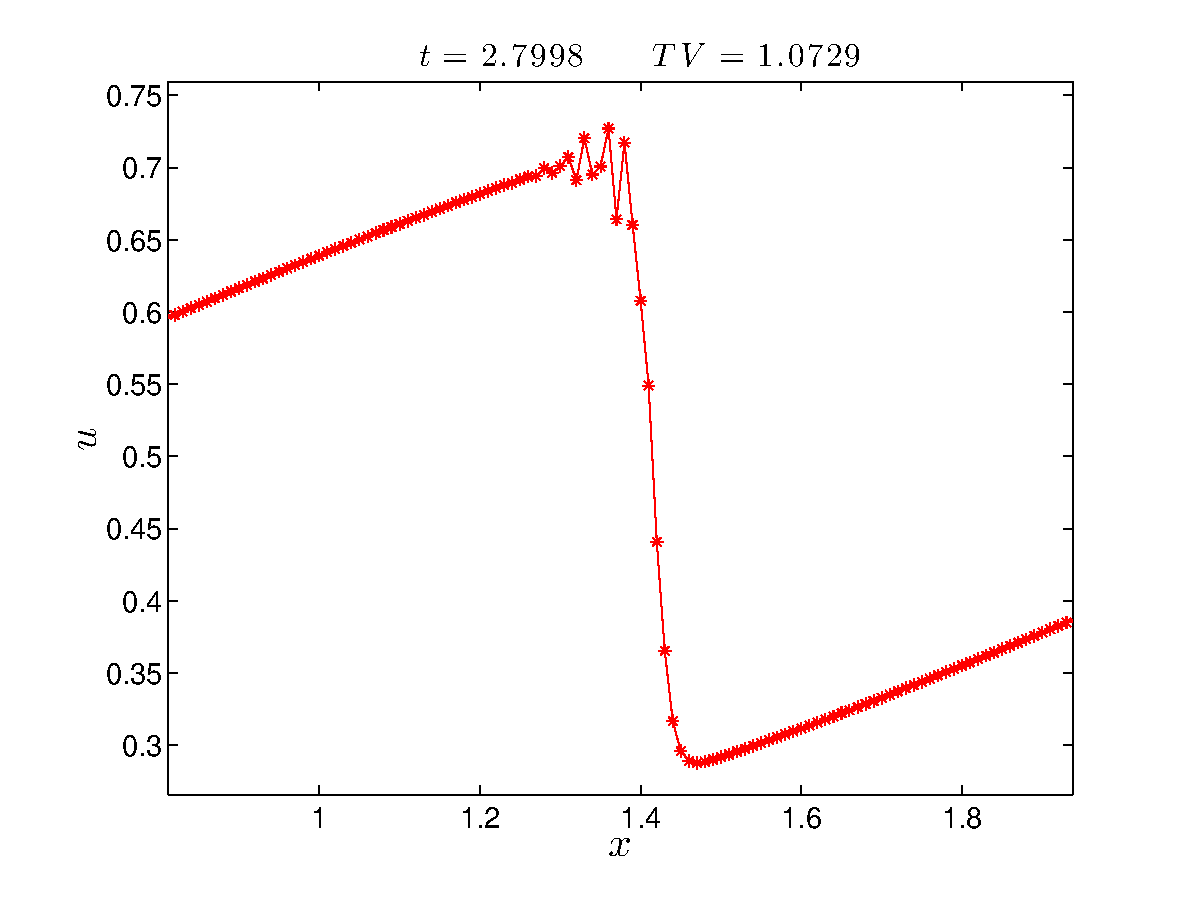
\includegraphics[width=0.5\textwidth]{Pictures/burgers_cont_no_tvd}}
    \caption{Solution of Burgers' equation with continuous initial data, using a 
    $TM^{n-2}R$ scheme, where $ M $ is SSPRK($10,4,2$). 
    The SSP coefficient is $\sspcoef = 6.0$. 
    Here $TV$ denotes the difference between the $TV$-norms of the final and 
    initial solution.
    A positive sign indicates a violation of the TVD condition.}
    \label{fig:burgers_cont}
\end{figure}

Burgers' equation was solved using an ESSPRK-scheme with time-step 
restriction $\Dt \leq \sigma{\Dt}_{\text{FE}}$, where $\sigma$ indicates the size 
of the time step. 
We integrate to time $t_{f} = 2.3$
\colintodo{double-check this $t_f$}
with $m = 256$ points in space.
Figure \ref{fig:burgers_cont} shows that if $\sigma$ stays below the SSP 
coefficient of the method $M$, then no oscillations are observed. 
If this stability limit is violated, then oscillations appear. 
\yiannistodo{Elaborate more: Sharpness of SSP coefficient} 
We were able to determine when exactly the nonlinear stability is not 
satisfied by computing the the total-variation (TV) norm at each step of the 
computation process. 
This indicates that the ESSPRK-scheme inherits the time-step restriction 
from the SSP coefficient of the main method $M$.


We also consider the Burgers' equation with discontinuous data
\begin{equation}\label{eq:burgers_discont_IC}
    u(0,x)  = \left\{
                \begin{array}{ll}
                  1, & \hbox{$0.5 \leq x \leq 1.5$} \\
                  0, & \hbox{otherwise.}
                \end{array}
              \right.
\end{equation}
Figure~\ref{fig:burgers_discont} shows the result of solving the 
discontinuous problem using an ESSPRK-scheme, where $M$ is an 
SSPRK($4,4,3$) method. 
The scheme preservers monotonicity in the TV-norm since the starting 
method $R$ is SSP. 
This is illustrated in Figure~\ref{fig:burgers_starting_method} in which 
the solution plotted after one step using methods $R$ and $S$ as the 
starting procedures.

\begin{figure}[t!]
    \centering
    \subfloat[$\sigma = 6.0$]{\label{fig:burgers_discont_a}
      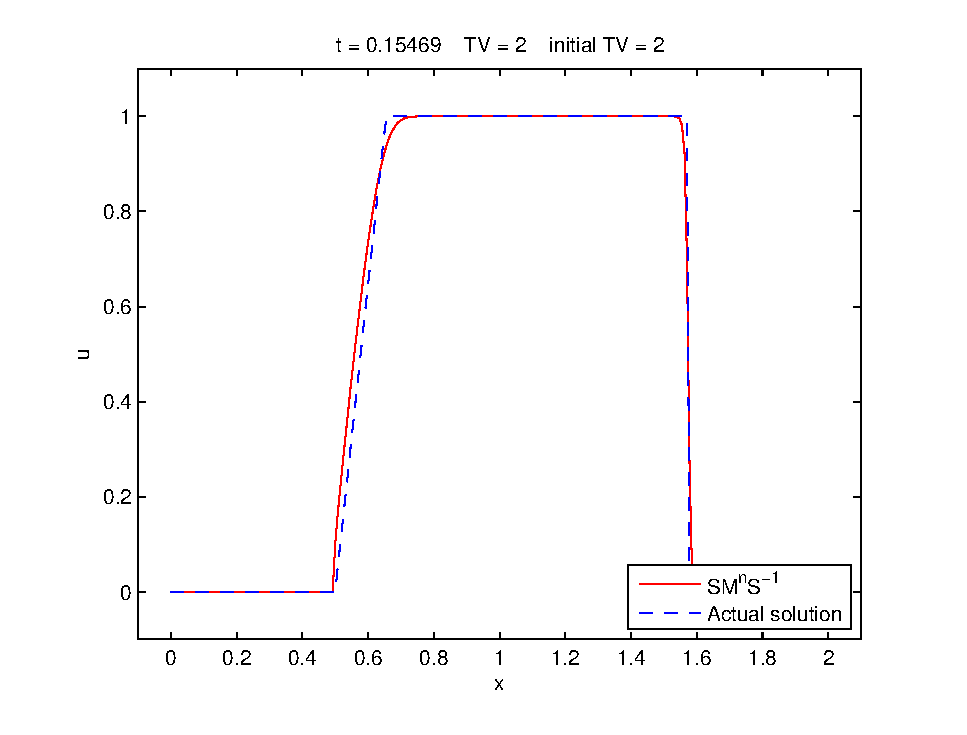
\includegraphics[width=0.5\textwidth]{Pictures/burgers_discont_tvd.eps}}
    \subfloat[$\sigma = 6.18$]{\label{fig:burgers_discont_a}
      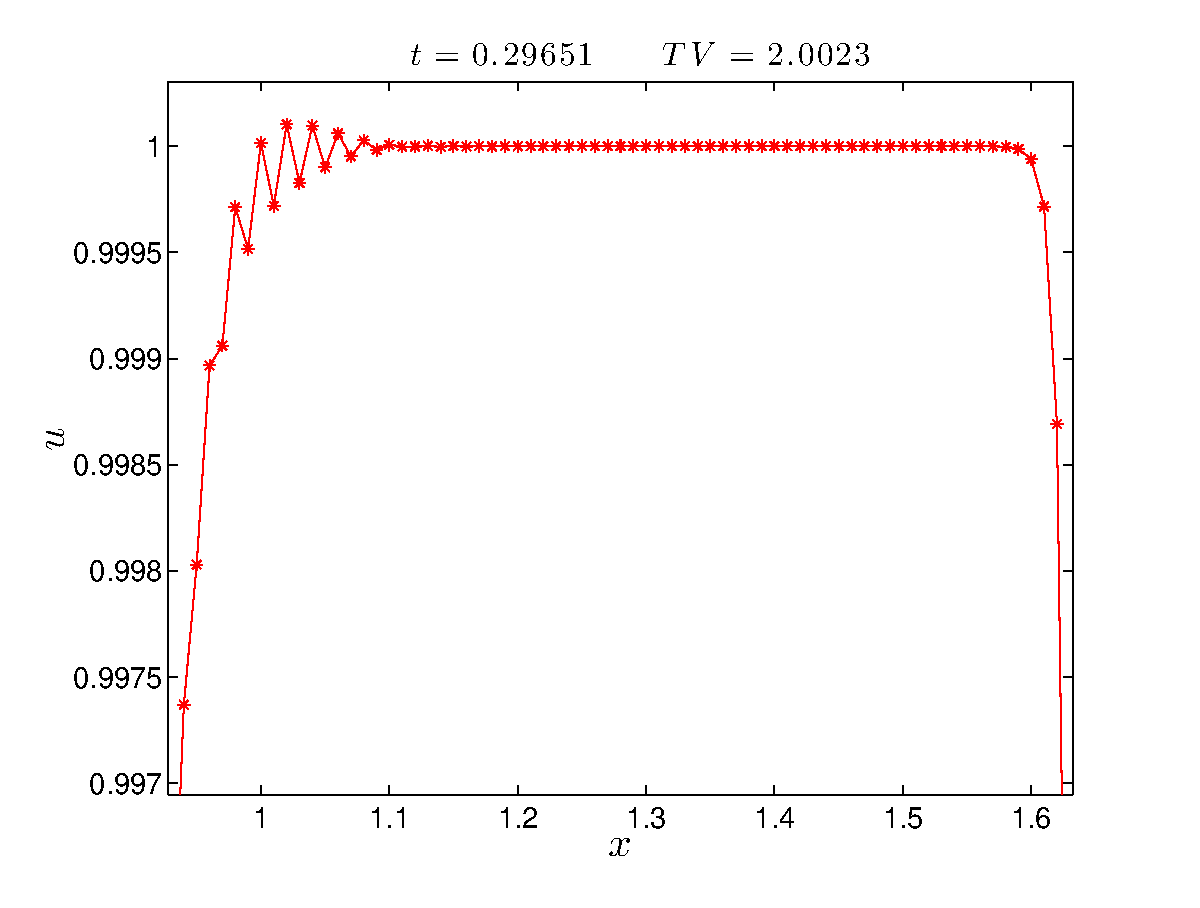
\includegraphics[width=0.5\textwidth]{Pictures/burgers_discont_no_tvd.eps}}
    \caption{Solution of Burgers' equation with discontinuous initial data, using a 
    $TM^{n-2}R$ scheme, where $M$ is SSPRK($10,4,2$) method. 
    The SSP coefficient is $ \sspcoef = 6.0$.
    Here $TV$ denotes the difference between the $TV$-norms of the final and 
    initial solution.
    A positive sign indicates a violation of the TVD condition.}
    \label{fig:burgers_discont}
\end{figure}

\begin{figure}[t!]
    \centering
	TODO
	\yianniscomment{This should be cut out since if we optimize directly for R and T, we are not mentioning S.}
    \caption{Solution of Burgers' equation with discontinuous initial data 
    after one step, using a $TM^{n-2}R$ scheme, where $M$ is an 
    SSPRK($5,4,2$) method. The solution is advanced one step by using (a) $R$ and 
    (b) $S$}
    \label{fig:burgers_starting_method}
\end{figure}

